\documentclass[a4paper, 12pt]{article}
\usepackage[utf8]{inputenc}
\usepackage[T1]{fontenc}
\usepackage[french]{babel}
\usepackage{graphicx}
\usepackage[hidelinks]{hyperref}
\usepackage[toc,page]{appendix}
\usepackage{float}
\usepackage{amsmath}
\usepackage{fancyhdr}
\pagestyle{fancy}

\cfoot{RedSquare}
\lhead{}
\chead{}
\rhead{}
\lfoot{}
\rfoot{\thepage}
\renewcommand{\footrulewidth}{0.4pt}
\renewcommand{\headrulewidth}{0pt}

\graphicspath{{./pictures/}}

\begin{document}

\begin{titlepage}
\begin{center}


\includegraphics[scale=0.25]{./TiltelPage/Logo}~\\[1cm]

\textsc{\LARGE UFR Sciences et Techniques  Besançon}\\[1.5cm]
Rapport\\
\textsc{Projet de Licence}

\newcommand{\HRule}{\rule{\linewidth}{0.5mm}}

\HRule \\[0.4cm]

{\huge \bfseries RedSquare}

\HRule \\[1.5cm]

\end{center}
\begin{minipage}{0.9\textwidth}
\begin{center} \large

\textsc{Lucas Grosjean, }
\textsc{Rémi Simonin, }
\textsc{Vincent Tourneret}
\textsc{et Florian Vetter}
\end{center}
\end{minipage}
\newline

\begin{center} \large
Tuteur de projet\\
\textsc{Julien Bernard}
\end{center}

\vfill

\begin{center}
{\large \today}
\end{center}

\end{titlepage}

\newpage
\section*{Introduction} 
\textbf{Un roguelike} est un jeu vidéo de type RPG(role playing game).
\\
D'un point de vue historique, le premier jeu de la lignée se nomme \textbf{Rogue}. Né en 1980, il donne lieu à plusieurs dizaines de successeurs qui ont repris les codes du genre.
\\
\\
Le sujet que nous avons choisi est d’implémenter un roguelike en solo ou ou en coopératif via une connexion réseau. Notre jeu s'appelle RedSquare. Ce nom  vient de la première fonctionnalité que nous avons du implémenter : faire bouger un carré rouge en réseau.
\\ 
L'objectif principal sera de parcourir un donjon le plus longtemps possible tout en essayant de ne pas mourir sous le coups des monstres rencontrés.
Les salles devront être créées au fur et à mesure que le joueur progresse. Ceci est appellé \textbf{génération procédurale} et c'est l'une des caractéristique fondamentale de ce type de jeu.
\\
Nous y trouvons également le \textbf{tour-par-tour}. Chaque personnage pourra éxecuter des actions uniquement quand c'est à lui de jouer, et celles-ci sont limités par des points d'action, qui empèchent par exemple des attaques trop nombreuses.
Chaque mort d'un joueur est définitive et il n'y a pas de système de sauvegarde. Lorsque un personnage quitte le jeu, la création d'une nouvelle partie implique une \textbf{remise à zéro} de son niveau et de son inventaire.
\\
Afin de présenter notre projet, nous commencerons par expliquer en détail les règles du jeu. Nous parlerons des différentes interractions qu'un utilisateur peut avoir avec le système ainsi que l'utilisation des classes au sein de celui-ci. Nous parlerons ensuite de nos implémentations ainsi que de nos choix techniques. Nous finirons par notre ressenti et de notre organisation pour ce projet. \textbf{Un roguelike} est un jeu vidéo de type RPG(role playing game).

\newpage
\tableofcontents
\newpage
\section{Spécifications et modélisation}
 \subsection{Règles du jeu}

Nous allons ici présenter l'utilisation de notre jeu.
Pour le lancer, l'utilisateur devra tout d'abord s'assurer qu'un serveur et bien lancé et qu'il est bien présent sur son réseau. Si ce n'est pas le cas, le programme enverra une erreur.
\\
Une fois le serveur en marche, le joueur lancera le programme client qui l'amenera directement sur un lobby qui permettra au joueur de choisir le jeu qu'il veut rejoindre et les joueurs déjà présents sur le serveur. 
\\
Une fois une séléctionnée/créée, vous aurez la possibilité de choisir une classe de personnage que vous jouerez tout au long de la partie.
\\
\\
Voir ImageClasseJoueur.
\\
\\
Une fois que le créateur de la partie décide qu'il y a assez de joueur, entre 1 et 9, il lance le jeu et les utilisateurs quitte le lobby pour la première salle de donjon.
\\
\\
Voir photo de la première salle du donjon
\\
\\
Chaque personnage est alors au niveau 1 étant donné qu'un roguelike  ne comporte pas de système de sauvegarde. 
Les tours de jeu sont définis par l'ordre dont les joueurs sont arrivés dans le salon. C'est donc au créateur d'éxécuter la première action. À chaque tour de jeu, une notification nous prévient que nous avons la possibilité de jouer.
\\
\\
imagePremierTour
\\
\\
Il aura alors le choix de ce déplacer, il pourra alors utilisé les flèches directionnelles, les touches z,q,s,d ou la souris. Celle-ci est le seul moyen de choisir une destination ne se trouvant pas sur les cases adjacentes à la position actuelle. Le chemin sera visible par un système de surbrillance des cases. Si une case que l'on choisie n'est pas une case sur laquelle nous pouvons nous trouver alors l'action ne sera pas déclenchée et le joueur sera obligé de choisir une nouvelle destination, une autre action ou alors il pourra passer son tour.
\\
\\
Voir photoSurbrillanceCase
\\
\\
Le personnage aura aussi la possibilité d'attaquer. Si un ennemi se trouve à proximité, l'utilisateur pourra le pointé avec sa souris. Si le curseur ne prend pas la forme d'une épée, c'est que le monstre ne se trouve pas dans l'aire de combat du personnage.
Le joueur aura le choix entre un attaque de base, que toutes les classes possèdent dés le départ, ou une attaque spéciale propre à chaque classe. Ces attaques consomment du mana qui permettra de ne pas abuser des sorts puissants. Une fois le mana épuisé, il faudra changer de niveau ou prendre une potion adéquate afin de le récupérer.
\\
\\
Voir photoCurseur
\\
\\
Il est important de savoir que chaque personnage peut attaquer plus ou moins loin selon son type de classe. Par exemple, le guerrier pourra attaquer uniquement les ennemis se toruvant sur les cases du haut, du bas et de coté tandis que le mage pourra attaquer en diagonales ou deux cases plus loin que sa position.
Certains ennemis sont plus difficiles à vaincre que d'autres. Il faut donc ne pas se précipiter et anticiper les attaques afin de perdre le moins de vi possible.
\\
\\
Voir tableau des monstres
\\
\\
Si un coffre se trouve à proximité, l'utilisateur pourra l'ouvrir et glisser les objets dans son inventaire. Pour savoir si le coffre peut s'ouvrir, une clé remplacera le curseur actuel. Cette action ne met pas fin au tour du joueur. Il pourra rechoisir une des deux actions précédentes à exécuter.
\\
\\
ImagedeCurseur et Imagenventaire
\\
\\
Un joueur peut tout de même effectué certaines actions même lorsque ce n'est encore pas à lui de jouer. Ces actions sont alors possibles à tout moment du jeu.
\\
Il pourra tout d'abord utiliser son inventaire. Pour l'ouvrir il appuiera sur la touche 'i'. Il aura la possibilité de s'équiper d'armes ou d'armures qui augmenteront ses performances. Il est aussi capable d'utiliser des potions qui lui augmenteront redonneront de la vie ou/et du mana ainsi qu'une amélioration d'attaque ou de défense. 
\\
\\
voirInventaire
\\
\\
Il peut également afficher la minimap en appuyant sur la touche "m". Celle-ci rendra compte de la disposition de l'étage ainsi que la position de ses équipers.
\\
\\
image minimap
\\
\\
Il pourra par ailleurs communiquer avec un autre utilisateur via l'utilisation du chat. Il aura le choix d'envoyer des messages globaux, pouvant être vu par tous ainsi que des messages privés, déstinés à un unique coéquipier. Le chat permet également de tenir compte de l'avancement du jeu étant donné que les messages provenant du système affiche les précédentes actions du jeu. Par exemple, la mort d'un adversaire sera visible par tous les joueurs.
\newpage

\subsection{Représentation UML}
\begin{figure}[H]
    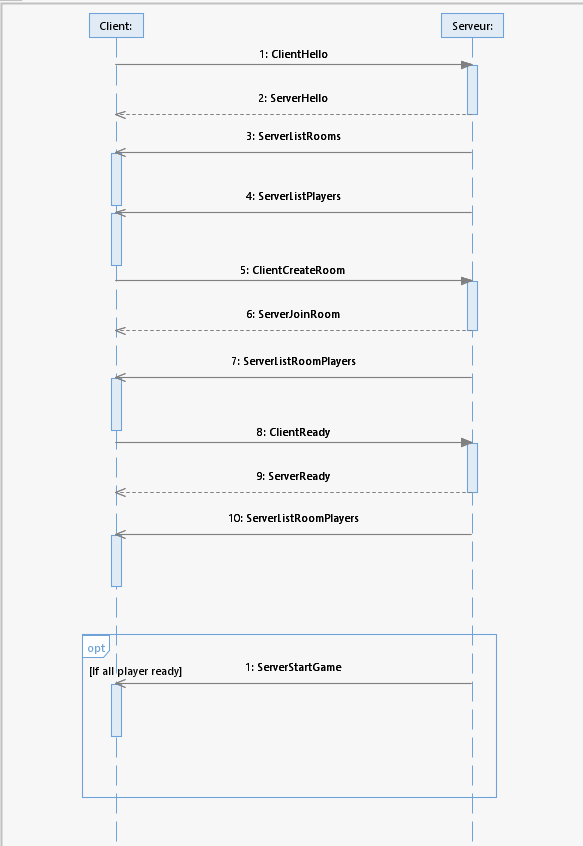
\includegraphics[scale=0.6]{./Diagramme/Connection}
    \caption{Protocole de connection}
\end{figure}
\newpage
\begin{figure}[H]
    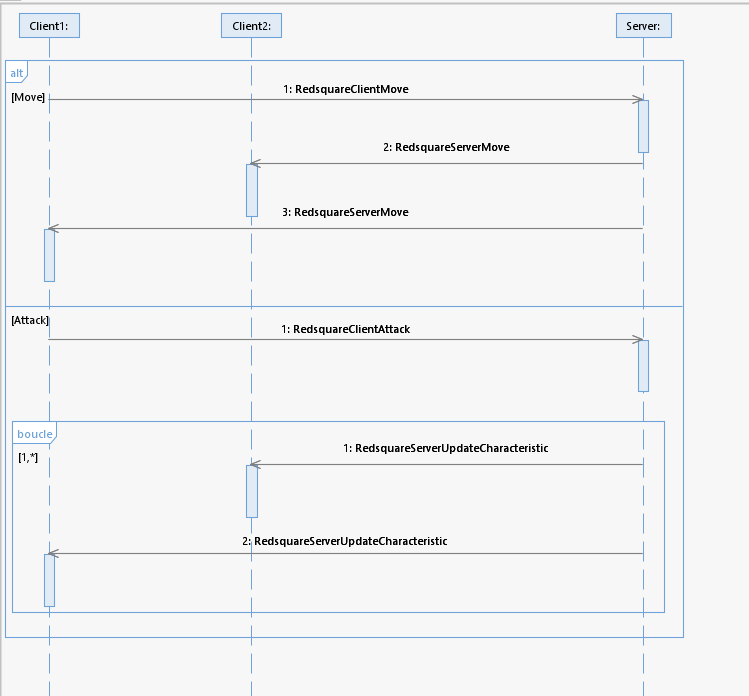
\includegraphics[scale=0.65]{./Diagramme/Deplacement}
    \caption{Protocole de deplacement}
\end{figure}
Lorsqu'un joueur fait un déplacement, il envoie le protocole "RedsquareClientMove" qui contient un vecteur, qui permet de savoir la direction du déplacement, le serveur regarde si les conditions sont toutes correct, si c'est le cas, le serveur envoie à tous les joueurs le paquet "RedsquareServerMove" avec le type d'entité, l'id de celui-ci et la position.
\newpage
\begin{figure}[H]
    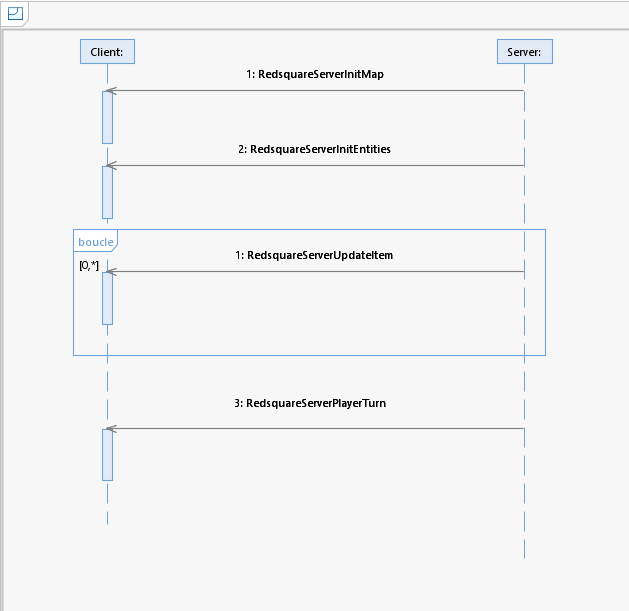
\includegraphics[scale=0.65]{./Diagramme/Jeu}
    \caption{Protocole d'initialisation du jeu}
\end{figure}
Lors de la connection, Nous devons d'abord envoyer la carte à tous les joueurs grace au paquet RedsquareServerInitMap. Ensuite nous devons envoyer toutes les entités créé au préalable lors de la generation dans le paquet "RedsquareServerInitEntities", qui contient un vecteur de structure qui contient toutes les donnés pour la création de l'entitié. Ensuite nous envoyons tous les items créé dans les différents objets de la carte avec le paquet "RedsquareServerUpdateItem". Et pour finir, nous envoyons le paquet "RedsquareServerPlayerTurn" au premier joueur qui doit jouer son tour.
\newpage
\begin{figure}[H]
    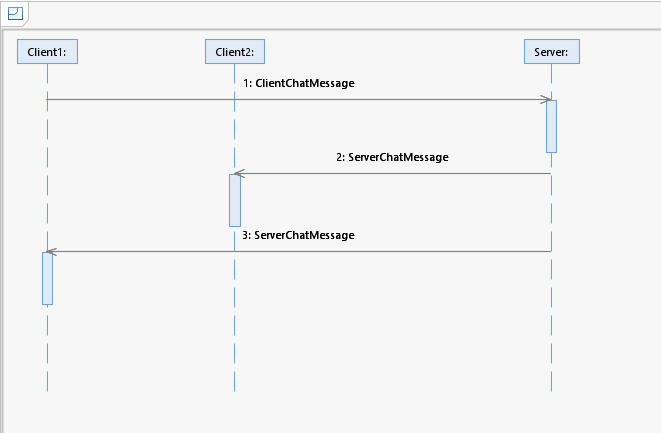
\includegraphics[scale=0.7]{./Diagramme/Chat}
    \caption{Protocole d'envoie d'un message}
\end{figure}
Lorsqu'un client envoie un message dans le chat, on envoie le paquet "ClientChatMessage" qui contient le message et aussi l'id du destinataire lors d'un message privé. Lorsque le serveur reçoit ce paquet, il envoie le paquet "ServerChatMessage" à tous les joueurs y compris l'envoyeur. Si c'était un message privé, seulement l'envoyeur et le destinatire recevrait le paquet.
\newpage

\subsection{Éléments de gameplay}
\subsection*{Personnages jouable}
\begin{center}
\begin{tabular}{ | c | c | c | }
	\hline
    Sprite & Nom & Particularités\\
    \hline
    
    
\includegraphics[scale=2.2]{./players/Magus} & Mage & Portée de 2 cases et dégats moyen\\
    \hline
    
    
\includegraphics[scale=1.9]{./players/WarriorNew} & Guerrier & Vie et défense élévés\\
    \hline
    
    
\includegraphics[scale=2.2]{./players/Rogue} & Assasin & Dégats élevés mais peu de défense\\
    \hline
    
    
\includegraphics[scale=2.2]{./players/Ranger} & Tireur & Portée de 3 cases mais peu de dégats\\
    \hline
    
    
\includegraphics[scale=1.9]{./players/Healer} & Prêtre & Portée de 2 cases et soins élevés\\
	\hline
\end{tabular}
\end{center}
\subsubsection*{Ennemies}
\begin{center}
\begin{tabular}{ | c | c | c | }
	\hline
    Sprite & Nom & Particularités\\
    
\includegraphics[scale=2]{./monsters/Orc} 
\includegraphics[scale=2]{./monsters/Mask}
    
\includegraphics[scale=1.5]{./monsters/SkeletonKnife} 
\includegraphics[scale=2]{./monsters/Zombie} & Tanks & Vie et défense élévés\\
    
    \hline
    
\includegraphics[scale=2]{./monsters/Swamp} 
    
\includegraphics[scale=1.4]{./monsters/Slime}
    
\includegraphics[scale=1.9]{./monsters/Spirit}
    
\includegraphics[scale=1.7]{./monsters/Bat} & Esprits & Dégats élevés mais peu de vie\\
   
    \hline
    
\includegraphics[scale=2]{./monsters/Demon}
\includegraphics[scale=2]{./monsters/Imp}
    
\includegraphics[scale=2]{./monsters/LilGob}
    
\includegraphics[scale=2]{./monsters/LilZombie} & Assasins & Dégats élevés mais peu de défense\\
    
    \hline
    
\includegraphics[scale=2]{./monsters/Lizard}
    
\includegraphics[scale=1.5]{./monsters/SkeletonMagus} 
    
\includegraphics[scale=1.5]{./monsters/Goblin}
    
\includegraphics[scale=2]{./monsters/Shaman} & Mages & Portée de 2 cases mais peu de dégats\\
	\hline
\end{tabular}
\end{center}
\subsection*{Sorts}
Il existe 18 sorts dans le jeu. Il y à plusieurs types de sort, comme des sorts de dégats, de soin et de boost. \\
Nous allons maintenant vous présenter 3 sorts : 

\begin{figure}[h]
\center

\includegraphics[scale=2]{./Spell/Basic1}\\
\caption{BasicAttack}
\label{fig:BasicAttack}
\end{figure}

La figure \ref{fig:BasicAttack} est l'attaque de base de chacun des personnages, cette attaque ne consomme pas de mana contrairement à tous les autres sorts.

\begin{figure}[h]
\begin{center}

\includegraphics[scale=2]{./Spell/Reaper1}\\
\caption{Reaper}
\label{fig:Reaper}
\end{center}
\end{figure}


La figure \ref{fig:Reaper} est un sort de zone qui va permettre à son lancer de taper toute les cases devant lui, ce sort coûte 7 point de mana.\\

\begin{figure}[h]
\center

\includegraphics[scale=7]{./Spell/DoubleStrike1} \\
\caption{DoubleStrike}
\label{fig:DoubleStrike}
\end{figure}

La figure \ref{fig:DoubleStrike} est un sort qui va frapper sa cible avec 2 attaques qui font chacune 70\% de dégat par rapport à l'attaque de base, ce sort coûte 5 point de mana\\

\subsubsection*{Objet}
Il existe dans RedSquare, plus de 135 équipements différents. Ces équipements et potions se trouvent dans les coffres que l'on peut trouver dans les salles du donjon. \\
Un joueur peut s'équiper d'une arme (épee, arc, bâton, livre de sort), d'un bouclier, d'un casque, d'un plastron, d'un pantalon et d'une paire de botte.
Il existe 15 type de chacune de ces pièces d'équipements avec chacunes des bonus différents, certaines pièce donnerons plus de vie alors que d'autre plus de défense.\\
Chacune de ses pièces d'équipement ont le même taux d'apparition dans un coffre, à la différence que tous les types d'équipement ne sont disponible qu'à partir de certains étages.
\\
Dans RedSquare il y a 8 types de potion et chacun de ses types de potion contient 3 tier, plus le tier est élevée plus la potion est efficace.\\
\begin{table}[h]
    \begin{tabular}{  | c | c | c | }
        \hline
        Potion de vie & Potion de mana & Potion d'énergie (vie + mana)\\
        \hline
        Boost de vie & Boost de mana & Boost d'attaque\\
        \hline
        Boost de défense & Boost d'expérience &\\
        \hline
    \end{tabular}
    \caption{Les différents type de potion dans RedSquare}
\end{table}

\subsection*{Inventaire}
\subsection*{Chat}
\subsection*{Salle de boss}

\section{Réalisation/Implémentation}
\subsection{Choix des technologies}
\subsubsection*{Interface réseau}
Nous avons dû faire un choix pour l'interface réseau que nous allons utiliser. Nous avons deux interfaces en concurences :\\
\begin{tabular}{ | c | c | }
    \hline
    Boost.Asio & gf::net \\
    \hline
    \begin{tabular}{ | c | c | }
        \hline
        Avantages & Inconvénients \\
        \hline
        Rapidité
        &
        Implémentation difficile\\
		\hline
		Beaucoup de documentation et d'aide en ligne
        &
        Utilisation de thread pour chaque connection\\
		\hline
    \end{tabular}
    &
    \begin{tabular}{ | c | c | }
        \hline
        Avantages & Inconvénients \\
        \hline
        Implementation simple 
        & 
        Lenteur \\
		\hline
		Selecteur de socket implémenté
        & 
        Moins d'aide en ligne \\
		\hline
    \end{tabular} \\
    \hline
\end{tabular}
Nous décidons de choisir gf::net, pour son selecteur de socket, qui nous facilite la tâche lors de l'implementation côté serveur.
\subsubsection*{Interface graphique}
Nous avions besoin de gérer les différentes interfaces
graphiques du jeu. Pour cela nous allons comparer les deux outils possibles que nous avons utilisé dans notre projet.\\

Le premier outil, est une classe nommée UI, apportait un rendu satisfaisant, directement implémenté dans gf elle était facile de compréhension et d'utilisation ce qui nous a fait gagner beaucoup de temps.
Mais cette classe apportait quelques incovénients, pour notre chat qui utilisait UI, le texte affiché
ne se retournais jamais a ligne, ce qui était vraiment problèmatique pour les
longs messages. Un autre inconvénient était la taille des fenètres lors du passage de petit a plein écran, en effet la taille de la fenètre crée ne changait pas alors que celle du jeu changait.
\\Le second outil, est une bibliothèque nommée Dear ImGui, apportait un rendu visuel vraiment agréable et nous permettait de répondre à tout les inconvénients de UI donc un retour à la ligne, un changement de taille de la fenètre, etc.ImGui offrait également bon nombre de fonctions nous permettant un rendu visuel personnalisé(arbres, textWrap...).
Les inconvénients de Dear ImGui, était que la bibliothèque n'était pas implémenté directement dans gf, ce qu'il la rendait plus difficle d'utilisation (pour la lié à tout notre jeu) et de compréhension.Il y avait aussi le fait qu'il n'était pas possible d'intégrer des images dans la fenètre utilisant ImGui. Un des plus gros inconvénient de ImGui était que l'on ne pouvait pas changer la taille du texte dans les fenètres ce qui nous limitaient lors du passage en pleine écran.\\

Après avoir analysé le pour et le contre nous avons donc décidé d'utiliser Dear ImGui, pour son aspect visuel et ImGui nous en offrait une de qualitée. ImGui nous permet également de résoudre les probèmes de UI et donc de pouvoir creer l'affichage graphique voulu.
\\
Protocole de connexion(avec un seul joueur)
(screnn ancien et nouveau chat)
\newpage
\subsection{Gameplay}
Peut être plus sur l’input en premier et que ensuite on fait dans le update ect ?
\newpage
\subsection{Génération du jeu}

\begin{figure}
\center
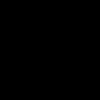
\includegraphics[width=10cm,height=6cm]{./Procedural/void}
\caption{Carte vide}
\label{vide}
\end{figure}

\begin{figure}
\center
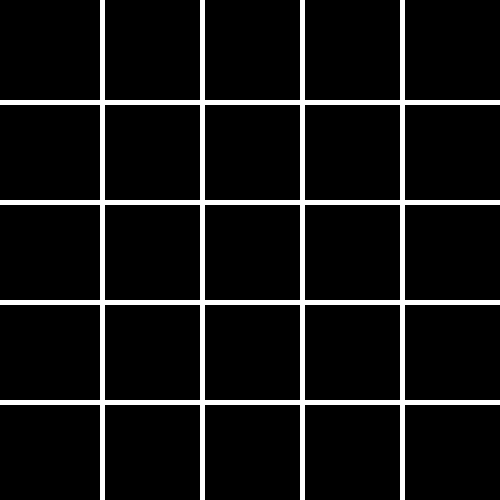
\includegraphics[width=10cm,height=6cm]{/Procedural/grid}
\caption{Grille}
\label{grid}
\end{figure}

\begin{figure}
\center
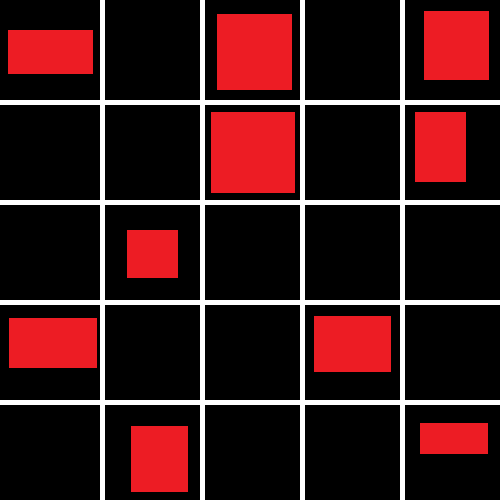
\includegraphics[width=10cm,height=6cm]{/Procedural/floor}
\caption{Génération du sol des salles}
\label{floor}
\end{figure}

\begin{figure}
\center
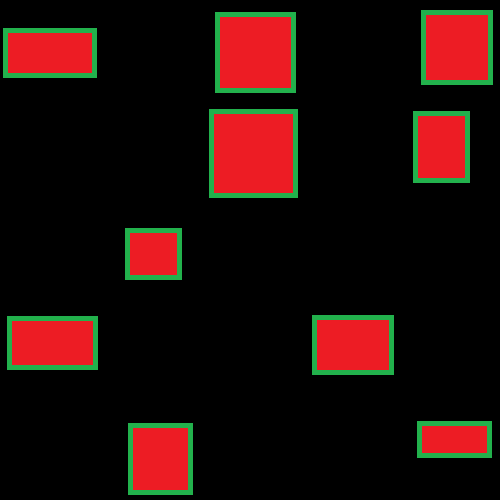
\includegraphics[width=10cm,height=6cm]{/Procedural/wall}
\caption{Ajout des murs}
\label{wall}
\end{figure}

\begin{figure}
\center
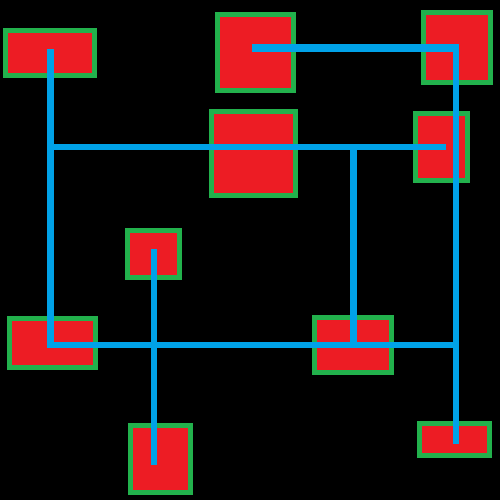
\includegraphics[width=10cm,height=6cm]{/Procedural/corridor}
\caption{Ajouts des couloirs}
\label{corridor}
\end{figure}

\begin{figure}
\center

\includegraphics[width=10cm,height=6cm]{/Procedural/stair}
\caption{Placement des meubles, monstres, escalier et joueurs}
\label{stair}
\end{figure}

La génération de la carte se déroule en plusieurs étapes: \\

La première étape consiste à dimensionner la zone jouable, c'est à dire les bornes de la carte. Dans notre jeu, tous les étages font 100 cases par 100 cases, comme on peut le voir que la Figure \ref{vide}.  \\

La seconde étape consiste à créer une grille sur la carte. Cette grille permet de découper la zone jouable en plusieurs carrées où l'on viendra générer les salles du donjon. Cette grille est visible sur la Figure \ref{grid}  \\

La troisième étape est la génération du sol des salles, ceci correspond à la Figure \ref{floor}. Nous tirons au sort plusieurs carrés où l'on va générer les salles, la plupart du temps nous générons dix salles dans l'étage. Nous sélectionnons un point au hasard dans le carré choisis pour accueillir une salle puis nous tirons au sort la largeur et la longueur (entre 6 et 26) de la futur salle. Si les bornes de la salle dépassent celles du carré alors nous tirons au sort une longueur et une largeur jusqu'à obtenir une salle qui rentre dans le carré. Nous stockons ensuite ces salles dans un vecteur4u qui stock les 4 coins des salles générées. Une fois les salles générées nous détruisons la grille. \\

La quatrième étape est celle où l'on va placer les murs autour des salles générées dans l'étape précédente, comme on peut le voir sur la Figure \ref{wall}. Pour cela nous utilisons le vecteur4u où nous avons stockées les sols des salles, nous parcourons ensuite une zone qui contient le sol de la salle et toute les cases adjacentes à ce sol. Nous plaçons ensuite des murs sur les cases adjacentes. Nous stockons les salles dans un autre vecteur4u. \\

La cinquième étape de cette génération procédurale est la génération des couloirs permettant de lier les salles entre elles. Pour se faire, nous sélectionnons 2 salles parmi celles que nous avons générées puis on prends le milieu de ces 2 salles qu'on relie grâce à la fonction computeRoute() de GF. Cette fonction implémente l'algorithme A* qui calcule le plus court chemin entre deux points et nous renvoie un vecteur contenant les cases du chemin le plus court. Nous parcourons alors ce vecteur pour y placer des cases de sol. Pour rendre la génération plus proche d'un donjon, nous sélectionnons un point adjacent au milieu de des salles que l'on va relier de la même manière que les deux premiers points. Cela permet d'obtenir des couloirs de deux de large. De la même façon que pour les salles, nous plaçons les murs sur les cases adjacentes au couloirs que l'on vient de générer. Nous exécutons ce processus jusqu'à l'avoir exécuté notre nombre de salle fois trois, ce qui nous permet d'être sûr d'avoir relié toute les salles entre elles. La Figure \ref{corridor} montre la carte après la génération de tous les couloirs.

La dernière étape de notre génération est le placement des éléments de jeu (meubles, monstres,escalier et les joueurs), ces différents éléments se trouve sur la Figure \ref{stair}. Nous parcourons une fois encore notre vecteur de salle et nous tirons au sort un thème. Ce thème nous permet de générer tel ou tel meuble en fonction du thème. Nous avons définis de nombreux thèmes tel que, une prison, une armurerie, une bibliothèque, une salle du trône, une salle avec des boîtes et des vases. Les meubles sont des entités destructibles qui ne possède qu'un point de vie. Leurs positions est aléatoire dans la salle, pour cela nous tirons une position dans la salle et nous vérifions que le meuble ne rentre pas en collision avec un autre. \\
Pour placer l'escalier nous tirons au sort une case vide dans une salle aléatoire et et on le place à cette position.
Nous plaçons ensuite les ennemis dans les salles de la même manière que les meubles. Nous tirons au sort les salles où les monstres vont apparaître, puis nous tirons une position vide dans cette salle pour y placer le monstre. \\
De la même manière, nous plaçons les joueurs à une position aléatoire dans une salle aléatoire. Nous faisons juste attention à ce que la salle contiennent un carré de trois par trois pour faire apparaître 9 joueurs (Nombre de joueurs maximale en multijoueur). \\
\begin{figure}
\center
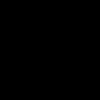
\includegraphics[width=10cm,height=6cm]{./Procedural/void}
\caption{Carte vide}
\label{vide}
\end{figure}

\begin{figure}
\center
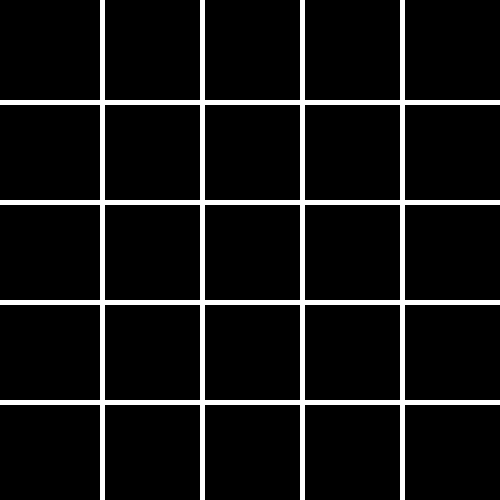
\includegraphics[width=10cm,height=6cm]{/Procedural/grid}
\caption{Grille}
\label{grid}
\end{figure}

\begin{figure}
\center
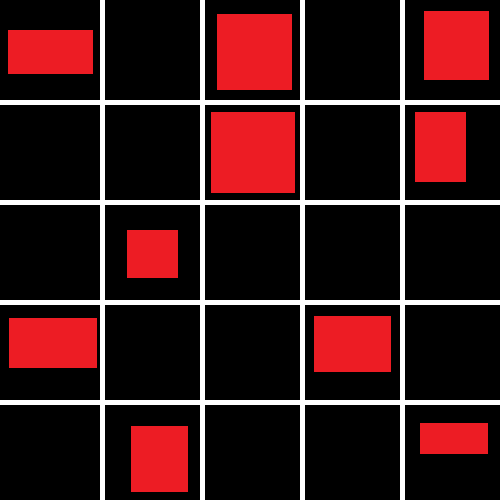
\includegraphics[width=10cm,height=6cm]{/Procedural/floor}
\caption{Génération du sol des salles}
\label{floor}
\end{figure}

\begin{figure}
\center
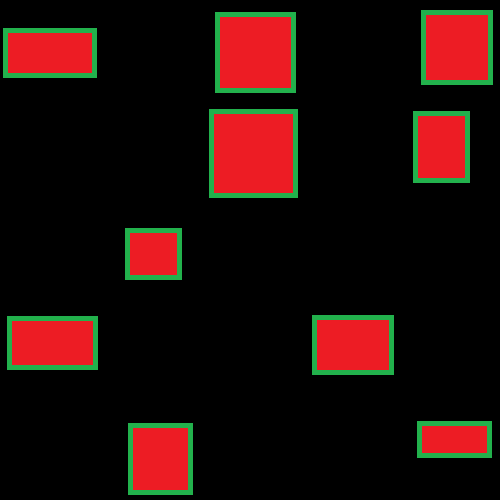
\includegraphics[width=10cm,height=6cm]{/Procedural/wall}
\caption{Ajout des murs}
\label{wall}
\end{figure}

\begin{figure}
\center
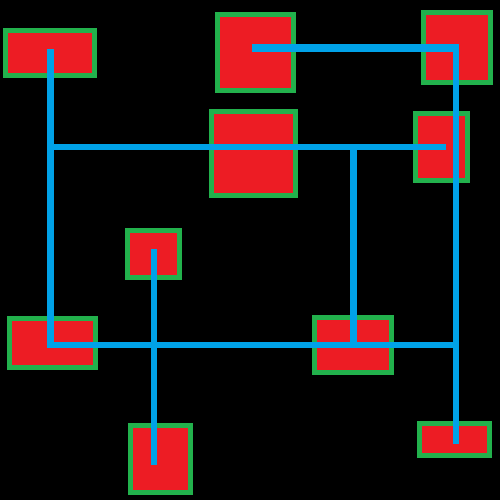
\includegraphics[width=10cm,height=6cm]{/Procedural/corridor}
\caption{Ajouts des couloirs}
\label{corridor}
\end{figure}

\begin{figure}
\center

\includegraphics[width=10cm,height=6cm]{/Procedural/stair}
\caption{Placement des meubles, monstres, escalier et joueurs}
\label{stair}
\end{figure}

La génération de la carte se déroule en plusieurs étapes: \\

La première étape consiste à dimensionner la zone jouable, c'est à dire les bornes de la carte. Dans notre jeu, tous les étages font 100 cases par 100 cases, comme on peut le voir que la Figure \ref{vide}.  \\

La seconde étape consiste à créer une grille sur la carte. Cette grille permet de découper la zone jouable en plusieurs carrées où l'on viendra générer les salles du donjon. Cette grille est visible sur la Figure \ref{grid}  \\

La troisième étape est la génération du sol des salles, ceci correspond à la Figure \ref{floor}. Nous tirons au sort plusieurs carrés où l'on va générer les salles, la plupart du temps nous générons dix salles dans l'étage. Nous sélectionnons un point au hasard dans le carré choisis pour accueillir une salle puis nous tirons au sort la largeur et la longueur (entre 6 et 26) de la futur salle. Si les bornes de la salle dépassent celles du carré alors nous tirons au sort une longueur et une largeur jusqu'à obtenir une salle qui rentre dans le carré. Nous stockons ensuite ces salles dans un vecteur4u qui stock les 4 coins des salles générées. Une fois les salles générées nous détruisons la grille. \\

La quatrième étape est celle où l'on va placer les murs autour des salles générées dans l'étape précédente, comme on peut le voir sur la Figure \ref{wall}. Pour cela nous utilisons le vecteur4u où nous avons stockées les sols des salles, nous parcourons ensuite une zone qui contient le sol de la salle et toute les cases adjacentes à ce sol. Nous plaçons ensuite des murs sur les cases adjacentes. Nous stockons les salles dans un autre vecteur4u. \\

La cinquième étape de cette génération procédurale est la génération des couloirs permettant de lier les salles entre elles. Pour se faire, nous sélectionnons 2 salles parmi celles que nous avons générées puis on prends le milieu de ces 2 salles qu'on relie grâce à la fonction computeRoute() de GF. Cette fonction implémente l'algorithme A* qui calcule le plus court chemin entre deux points et nous renvoie un vecteur contenant les cases du chemin le plus court. Nous parcourons alors ce vecteur pour y placer des cases de sol. Pour rendre la génération plus proche d'un donjon, nous sélectionnons un point adjacent au milieu de des salles que l'on va relier de la même manière que les deux premiers points. Cela permet d'obtenir des couloirs de deux de large. De la même façon que pour les salles, nous plaçons les murs sur les cases adjacentes au couloirs que l'on vient de générer. Nous exécutons ce processus jusqu'à l'avoir exécuté notre nombre de salle fois trois, ce qui nous permet d'être sûr d'avoir relié toute les salles entre elles. La Figure \ref{corridor} montre la carte après la génération de tous les couloirs. \\

La dernière étape de notre génération est le placement des éléments de jeu (meubles, monstres,escalier et les joueurs), ces différents éléments se trouve sur la Figure \ref{stair}. Nous parcourons une fois encore notre vecteur de salle et nous tirons au sort un thème. Ce thème nous permet de générer tel ou tel meuble en fonction du thème. Nous avons définis de nombreux thèmes tel que, une prison, une armurerie, une bibliothèque, une salle du trône, une salle avec des boîtes et des vases. Les meubles sont des entités destructibles qui ne possède qu'un point de vie. Leurs positions est aléatoire dans la salle, pour cela nous tirons une position dans la salle et nous vérifions que le meuble ne rentre pas en collision avec un autre. \\
Pour placer l'escalier nous tirons au sort une case vide dans une salle aléatoire et et on le place à cette position.
Nous plaçons ensuite les ennemis dans les salles de la même manière que les meubles. Nous tirons au sort les salles où les monstres vont apparaître, puis nous tirons une position vide dans cette salle pour y placer le monstre. \\
De la même manière, nous plaçons les joueurs à une position aléatoire dans une salle aléatoire. Nous faisons juste attention à ce que la salle contiennent un carré de trois par trois pour faire apparaître 9 joueurs (Nombre de joueurs maximale en multijoueur).
\newpage
\subsection{Sérialisation}
La sérialisation utilisé dans notre projet est celle implémentée dans gf, cela nous à fait gagner du temps car nous n'avons pas eu à la faire nous meme.
\section{Conclusion}
\subsection{Aspect gestion de projet}
Etant 4 dans notre groupe de projet et de groupe de td, il nous fallait
mettre en place des solutions pour nous permettre de travailler rapidement et
éfficacement. Il nous fallait donc un outil de developpement collaboratif nous
permettant de partager notre travail avec les autres. Nous avons fait le choix
d’utiliser github qui est un service web d’hébergement et de gestion de
développement de logiciels, lié à GitHub Desktop sur nos machines il était
facile de partager son code avec les autres où de gérer d’evntuel conflit dans
notre code.\\ 

Pour communiquer entre nous à distance nous avons crée un groupe
messenger et un serveur discord, nous permettant de discuter du projet sans
être a coté les uns des autres. Lorsque nous voulions travailler depuis chez
nous, tout en voulant discuter du projet nous utilisions notre serveur discord.
Notre serveur nous permettait de réaliser des scéances de ouijas (terme que
nous utilisions pour définir nos soirées de codes tard le soir).
Pour pouvoir travailler entre nous côte à côte, on se rejoignais dans une sale
lorsque nous n’avions pas cour où les mardis soir prendant les scéances du dps
(club de jeu vidéo).\\

Lorsque nous avions un problème sur notre implémentation où sur nos
choix, nous allions directement demander à notre tuteur, nous permettant de
résoudre rapidement nos problèmes. Les reunions était importante et nous
permettaient de faire le point sur notre code avec notre tuteur et de discuter
de potentiel problème ou évolution du projet.\\
\newpage
\subsection{Perspectives d’amélioration}
Comme tout jeu vidéo,on pourait ajouter encore beaucoup d’options pour
améliorer la qualité du jeu. Comme de nouveau personnage, des sorts, des
items... On pourait ajouter de vrai boss dans les salles afin de créer de
véritable palliers de jeu et ainsi marqué une sorte de progression. De nouveaux
éléments de jeu tel que par exemple une monnaie dans le jeu couplé a une
boutique par étage nous permettant d’acheter des items ou bien de les vendres
dynamiserais le jeu. Nous avions également envisagé de créer un système de
sauvegardes des scores.

Au niveau de la génération procédurale de salle dans le donjon, nous aurions
pu créer plus de modèles de salles pour améliorer l’aspect graphique du jeu.
Au niveau des textures, la taille des textures étaient en 32x32. Ce choix de
base nous a par la suite limité dans notre volonté de rendre le jeu plus
agréable visuellement.
\newpage
\subsection{Synthèse}
Synthèse : projet trop facile
\newpage

\listoffigures
\end{document}